\chapter{Fundamental Groups}\label{chapter:fundamental.groups}

\section{Homotopy}
Continuous maps \(f, g \colon X \to Y\) between topological spaces \(X, Y\) are \emph{homotopic}\define{homotopic} if there is a \emph{homotopy}\define{homotopy} between them, i.e. a map \(F \colon [0,1] \times X \to Y\), denoted by \(F_s(x)\) instead of \(F(s,x)\), so that \(F_0=f\) and \(F_1=g\).
If there is a subset \(X_0 \subset X\) on which \(f=g\), \(f\) is \emph{homotopic} to \(g\) \emph{relative}\define{homotopy!relative}\define{relative homotopy} to \(X_0\) if there is a homotopy \(F\) between \(f\) and \(g\) so that \(F_s\of{x}=f(x)\) for all \(x \in X_0\).
A map is \emph{null homotopic}\define{null homotopic} if it is homotopic to a constant map, i.e. a map whose image is a single point.
\begin{problem}{covering.spaces:homotopic}
Prove that the relation of being homotopic relative to some set is an equivalence relation.
\end{problem}
Given points \(x_0, x_1 \in X\), a \emph{path}\define{path} from \(x_0\) to \(x_1\) is a continuous map \(x \colon [0,1] \to X\) so that \(x(0)=x_0\) and \(x(1)=x_1\), i.e. a map \(x \colon \pr{[0,1],0,1} \to \pr{X,x_0,x_1}\).
We often omit to write the expression ``relative to \(\Set{0,1}\)'' when discussing homotopies of paths, and the reader will have to decide when we should have written that expression.

Intuitively, a homotopy between paths looks something like
\begin{center}
\documentclass[tikz]{standalone}
\usetikzlibrary{arrows,calc,shapes,decorations.pathreplacing}
\begin{document}
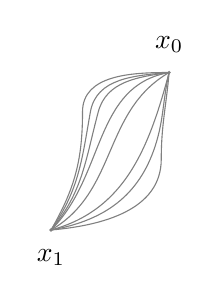
\begin{tikzpicture}[scale=.5]
%  \node at (0,0) {$F : I \times I \rightarrow X$};
\fill[gray] (6,0) circle (1.3pt);
  \node[label=below:$x_1$]  (x1) at (6,0)  {}; %{$\bullet$};
\fill[gray] (9,4) circle (1.3pt);
  \node[label=above:$x_0$]  (x0) at (9,4)  {}; % {$\bullet$};  
%  \node  at (9.5,2)  {$\subset X$}; 
  \draw[gray] (x1.center) to [out=5,in=-90]++(2.8,1.8) to[out=90,in=-95](x0.center);
  \draw[gray] (x1.center) to [out=10,in=-110]++(2.6,2) to[out=70,in=-103](x0.center); 
  \draw[gray] (x1.center) to [out=15,in=-105](x0.center);
  \draw[gray] (x1.center) to [out=30,in=-150](x0.center);
  \draw[gray] (x1.center) to [out=45,in=-170](x0.center); 
  \draw[gray] (x1.center) to [out=50,in=-105]++(1.2,3)to [out=75,in=-172](x0.center); 
  \draw[gray] (x1.center) to [out=55,in=-100]++(1.0,3) to[out=80,in=-175](x0.center); 
  \draw[gray] (x1.center) to [out=60,in=-90]++(0.8,3) to[out=90,in=-180] (x0.center);
%  \begin{scope}[every node/.style={draw, anchor=text, rectangle split,
%    rectangle split parts=7,minimum width=2cm}]
%    \node (R) at (2,4){ \nodepart{two} \nodepart{three}
%    \nodepart{four}$I\times I$\nodepart{five}\nodepart{six}\nodepart{seven}};
%  \end{scope}
%  \draw[decorate,decoration={brace,mirror,raise=6pt,amplitude=10pt}, thick]
%    (R.north west)--(R.south west) ;
%  \draw[decorate,decoration={brace,raise=6pt,amplitude=10pt}, thick]
%    (R.north east)--(R.south east); 
%  \draw[->] ($(R.west)+(-20pt,0)$) to[out=-180,in=240] ++(0,2)
%    to [out=60,in=120]node[above,midway]{$F(0,t_2)$}(x0) ; 
%  \draw[->] ($(R.north)+(0,10pt)$) to [out=60,in=120]
%    node[above,midway]{$\beta \simeq \alpha$} ++(4.5,-1) ; 
%  \draw[->] ($(R.east)+(20pt,0)$)  to [out=0,in=140]
%    node[right,midway]{$F(1,t_2)$}(x1) ; 
%  \draw[->] ($(R.south)+(0,-20pt)$)  to [out=-85,in=-30]
%    node[below,midway]{$\alpha$}++(7,0) ;    
\end{tikzpicture}
\end{document}

\end{center}
\begin{problem}{covering.spaces:reparam}
Take two paths \(x, y \colon [0,1] \to X\) for one is a \emph{reparameterisation},\define{reparameterisation} of the other, i.e. there is a continuous map \(\tau \colon [0,1] \to [0,1]\) so that \(y \circ \tau = x\) with \(\tau(0)=0\) and \(\tau(1)=1\).
Prove that \(x\) is homotopic to \(y\) relative to \(\Set{0,1}\).
\end{problem}
\begin{answer}{covering.spaces:reparam}
Let \(F_s(t)=x((1-s)t+s\tau(t))\).
\end{answer}
\begin{lemma}\label{lemma:pick.times}
Cover a topological space \(X\) in open sets \(X_a \subset X\).
Take a path \(x \colon [0,1] \to X\).
Then there are real numbers \(0=t_0 < t_1 < \dots < t_n=1\) so that \(x(t)\) stays in one open set \(X_{a_i}\) for \(t_i \le t \le t_{i+1}\).
\end{lemma}
\begin{proof}
Each point of \([0,1]\) lies in an open interval lying entirely inside one \(x^{-1}X_a\).
Replace that open interval with a smaller open interval: each point of \([0,1]\) lies in an open interval whose closure lies entirely inside one \(x^{-1}X_a\).
Since \([0,1]\) is compact, finitely many such open intervals cover \([0,1]\).
Take the endpoints of those intervals: \(0=t_0 < t_1 < \dots < t_n=1\).
\end{proof}

\section{Some inessential differential geometry}
Think of Euclidean space of dimension \(n\) as having \(n\) coordinates: 
\[
x=(x_1,\dots,x_n).
\]
An \(n\)-dimensional  \emph{manifold}\define{manifold} is a subset of Euclidean space \(\R{n+k}\), locally expressed as the graph of \(k\) of the coordinates as smooth functions of the other \(n\) coordinates.
An \(n\)-dimensional  \emph{manifold with corners}\define{manifold with corners} is a subset of Euclidean space \(\R{n+k}\), locally expressed as the graph of \(k\) of the coordinates as smooth functions of the other \(n\) coordinates, constrained to be inside an \(n\)-dimensional box.
A \emph{surface}\define{surface} is a \(2\)-dimensional manifold (perhaps with corners).
A continuous map of manifolds is \emph{smooth} if it is smooth as a map of those coordinates.
We won't prove:
\begin{theorem}
Every continuous map of manifolds is homotopic to a smooth map.
\end{theorem}
\begin{lemma}
Any path \(x \colon [0,1] \to M\) in a manifold (perhaps with corners) \(M\) is homotopic relative to \(\Set{0,1}\) to a smooth path.
\end{lemma}
\begin{proof}
If \(M=\R{n}\), and \(x \colon [0,1] \to M\) is a path then let \(y(t)=(1-t)x(0)+tx(1)\) and let \(F(s,t)=(1-s)x(t)+sy(t)\).
More generally, the same trick works for \(M\) any convex domain in \(\R{n}\), and in particular for \(M\) a box.

Suppose next that we have a path \(x(t)\) in a box \(M\), and we want to smooth out that path only inside some interval \(a < t < b\).
Take a smooth increasing function \(h(t)\) equal to \(0\) in a small neighborhood of \(a\), and equal to \(1\) in a small neighborhood of \(b\).
Let
\[
y(t) =
\begin{cases}
x(t), & \text{ if \(0 \le t \le a\)}, \\
(1-h(t))x(a)+h(t)x(b), & \text{ if \(a \le t \le b\)}, \\
x(t), & \text{ if \(b \le t \le 1\)}.
\end{cases}
\]
and let
\[
F(s,t)=(1-s)x(t)+sy(t).
\]

Cover \(M\) in open sets, each a graph over a convex open set in a box in \(\R{n}\).
Apply lemma~\vref{lemma:pick.times} to split \(x(t)\) into intervals on which it stays in these open sets.
On each interval, we use the first trick to smooth \(x\).
This done, \(x\) is now piecewise smooth.
We use the second trick near each corner to smooth out corners.
\end{proof}

\section{Loops}
A \emph{loop}\define{loop} is a path \(x \colon [0,1] \to X\) with \(x(0)=x(1)\).
Given a path \(x\) from \(x_0\) to \(x_1\) and a path \(y\) from \(x_1\) to \(x_2\), define a path \(x*y\) from \(x_0\) to \(x_2\) by
\[
(x*y)(t) =
\begin{cases}
x(2t), & \text{if \(0 \le t\le \frac{1}{2}\)}, \\
y(2t-1), & \text{if \(\frac{1}{2} \le t\le 1\)}.
\end{cases}
\]
and define \(\bar{x}(t)=x(1-t)\).
Also, for any point \(x_0\), define the null path \(x(t)=x_0\) for \(0 \le t \le 1\) which we just denote by \(x_0\).

If you have two paths and I have two paths, with homotopies fixing endpoints between your first and my first, and between your second and my second, then we can make a homotopy between paths glued together:
\begin{center}
\documentclass[tikz]{standalone}
\usetikzlibrary{arrows,calc,shapes,decorations.pathreplacing}
\begin{document}
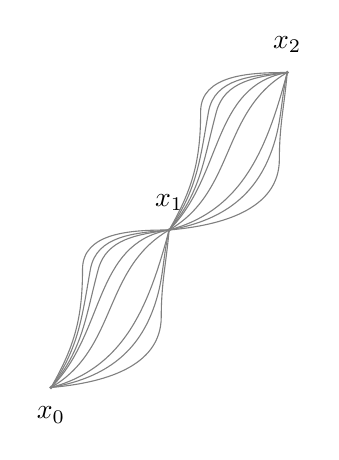
\begin{tikzpicture}[scale=.5]
\fill[gray] (6,0) circle (1.3pt);
  \node[label=below:$x_0$]  (x1) at (6,0)  {}; % {$\bullet$};
  \fill[gray] (9,4) circle (1.3pt);
  \node[label=above:$x_1$]  (x0) at (9,4)  {}; % {$\bullet$};  
%  \node[label=above:$x_1$]  (x0) at (9,4)  {$\bullet$};  
  \draw[gray] (x1.center) to [out=5,in=-90]++(2.8,1.8) to[out=90,in=-95](x0.center);
  \draw[gray] (x1.center) to [out=10,in=-110]++(2.6,2) to[out=70,in=-103](x0.center); 
  \draw[gray] (x1.center) to [out=15,in=-105](x0.center);
  \draw[gray] (x1.center) to [out=30,in=-150](x0.center);
  \draw[gray] (x1.center) to [out=45,in=-170](x0.center); 
  \draw[gray] (x1.center) to [out=50,in=-105]++(1.2,3)to [out=75,in=-172](x0.center); 
  \draw[gray] (x1.center) to [out=55,in=-100]++(1.0,3) to[out=80,in=-175](x0.center); 
  \draw[gray] (x1.center) to [out=60,in=-90]++(0.8,3) to[out=90,in=-180] (x0.center);
\begin{scope}[shift={(3,4)}]
\fill[gray] (6,0) circle (1.3pt);
  \node%[label=below:$x_1$]  
  	(x1) at (6,0) {};%  {$\bullet$};
%  \node[label=above:$x_2$]  (x0) at (9,4)  {$\bullet$};  
\fill[gray] (9,4) circle (1.3pt);
  \node[label=above:$x_2$]  (x0) at (9,4)  {}; % {$\bullet$};  
  \draw[gray] (x1.center) to [out=5,in=-90]++(2.8,1.8) to[out=90,in=-95](x0.center);
  \draw[gray] (x1.center) to [out=10,in=-110]++(2.6,2) to[out=70,in=-103](x0.center); 
  \draw[gray] (x1.center) to [out=15,in=-105](x0.center);
  \draw[gray] (x1.center) to [out=30,in=-150](x0.center);
  \draw[gray] (x1.center) to [out=45,in=-170](x0.center); 
  \draw[gray] (x1.center) to [out=50,in=-105]++(1.2,3)to [out=75,in=-172](x0.center); 
  \draw[gray] (x1.center) to [out=55,in=-100]++(1.0,3) to[out=80,in=-175](x0.center); 
  \draw[gray] (x1.center) to [out=60,in=-90]++(0.8,3) to[out=90,in=-180] (x0.center);
\end{scope}
\end{tikzpicture}
\end{document}

\end{center}
Hence gluing paths together commutes with homotopy relative to \(\set{0,1}\).
\begin{problem}{covering.spaces:associative}
For any three paths \(x, y, z\), if \((x*y)*z\) is defined then so is \(x*(y*z)\), and vice versa, and they are homotopic relative to \(\Set{0,1}\).
\end{problem}
\begin{problem}{covering.spaces:inverse}
For any path \(x\), the path \(x*\bar{x}\) is homotopic to \(x(0)\)  relative to \(\Set{0,1}\) while \(\bar{x}*x\) is homotopic to \(x(1)\) relative to \(\Set{0,1}\).
\end{problem}
Therefore, for any topological space \(X\) and point \(x_0 \in X\), the homotopy classes of loops relative to \(\Set{0,1}\) form a group, called the \emph{fundamental group}\define{fundamental!group} of \(X\) and denoted \(\fundamentalGroup{X,x_0}\).\Notation{p1M}{\fundamentalGroup{X,x_0}}{fundamental group}

\begin{problem}{covering.spaces:conjugacy}
If \(x_0,x_1 \in X\) are two points connected by a path \(x\), then any loop \(y\) at \(x_0\) has an associated loop \(\bar{x} * \pr{y * x}\) at \({x_1}\). 
Prove that the homotopy class of \(\bar{x} * \pr{y * x}\) in \(\fundamentalGroup{X,x_0}\) depends only on the homotopy class of \(y\) in \(\fundamentalGroup{X,x_1}\), and that this gives an isomorphism of groups
\[
\fundamentalGroup{X,x_0} \to \fundamentalGroup{X,x_1}.
\]
\end{problem}

A topological space \(X\) is \emph{path connected}%
\define{path connected}%
\define{connected!path}
if any two points of \(X\) are the endpoints of a path in \(X\).
If \(X\) is path connected, then we usually ignore the point \(x_0\) and write \(\fundamentalGroup{X}\) instead of \(\fundamentalGroup{X,x_0}\), even though this is not strictly speaking well defined.
A path connected topological space \(X\) is \emph{simply connected}\define{simply connected}\define{connected!simply} if \(\fundamentalGroup{X}=\left\{1\right\}\).
\begin{example}
A \emph{star shaped set}\define{star shaped} is a set \(X \subset \R{n}\) so that there is some point \(x_0 \in X\) so that for every point \(x_1 \in X\), the line segment from \(x_0\) to \(x_1\) lies entirely in \(X\).
\begin{center}
\documentclass[border=10pt]{standalone}
\usepackage{pgfplots}
\pgfplotsset{compat=1.8}
\usepgfplotslibrary{polar}
\begin{document}
\begin{tikzpicture}
	\begin{polaraxis}[xtick=\empty,ytick=\empty,mark=none,draw=white,opacity=0,thin,width=3cm]
	\addplot+[mark=none,domain=0:360,samples=1000,draw=gray!50,fill=gray!20,opacity=1] 
		{2-sqrt(sqrt((abs(sin(3*x)))))+cos(9*x)*cos(9*x)*cos(9*x)*cos(9*x)}; 
	% the expression is the RADIUS
	\end{polaraxis}
\end{tikzpicture}
\end{document}

\end{center}
In other words, \(X\) admits the homotopy \(F \colon (s,x) \in [0,1] \times X \mapsto x_0+s\pr{x-x_0} \in X\).
Clearly \(\fundamentalGroup{X}=\Set{1}\) is the trivial group, where \(1\) is the constant path \(x_0\).
In particular, \(\fundamentalGroup{\R{n}}=\Set{1}\).
\end{example}
\begin{example}
For the circle \(S^1\), take any path \(z(t)=x(t)+iy(t))\) on \(S^1\) and write it as \(z(t)=e^{i\theta(t)}\) using trigonometry to prove that one can continuously pick out a value of \(\theta(t)\) for any continuous \(z(t)\).
The number 
\[
n(z) \defeq \frac{1}{2\pi} \pr{\theta(1)-\theta(0)}
\]
is an integer, since \(z\) is periodic.
Suppose that two loops \(z_0(t)\) and \(z_1(t)\) have the same values of \(n\of{z_0}=n\of{z_1}\) and start (and thus end) at the same point of \(S^1\), say at \(e^{i \alpha_0}\).
Pick continuous angles \(\theta_0(t), \theta_1(t)\) with \(\theta_0(0)=\theta_1(0)=\alpha_0\) and 
\[
z_0(t)=e^{i\theta_0(t)}, z_1(t)=e^{i \theta_1(t)}.
\]
Clearly 
\[
\theta_0(1)=\theta_1(1).
\]
Let
\[
\theta_s(t) = (1-s)\theta_0(t)+s\theta_1(t)
\]
and 
\[
z_s(t) = e^{i\theta_s(t)},
\]
a homotopy.
Therefore \(\fundamentalGroup{S^1}=\Z{}\), identifying the homotopy class of a loop \(z\) with the number \(n(z)\).
\end{example}
\begin{example}
For an annulus 
\[
A\defeq\Set{x \in \R{n}|r_0 < \norm{x} < r_1},
\]
the map 
\[
F_s(x)=\frac{x}{(1-s)+s\norm{x}}
\]
retracts the annulus to the unit sphere, and retracts paths on the annulus to those on the sphere, homotopies on the annulus to homotopies on the sphere, so that \(\fundamentalGroup{A}=\fundamentalGroup{S^{n-1}}\).
\end{example}
\begin{example}
It turns out to be more difficult to find the fundamental group of the plane punctured at two points, or at three points, etc.
\end{example}
\begin{example}
The spaces \(\R{}\) and \(\R{2}\) are not homeomorphic, as \(\R{}\) becomes path disconnected when we remove any point, while \(\R{2}\) does not.
\end{example}
\begin{example}
The spaces \(\R{2}\) and \(\R{3}\) are not homeomorphic, as \(\R{2}\) punctured at any point has fundamental group \(\Z{}\), while \(\R{3}\) punctured at any point remains simply connected.
\end{example}
\begin{exampleAndImage}{2cm}
The Hawaiian earring has a very complicated and uncountable fundamental group.
\tcblower
\documentclass[tikz]{standalone}
\begin{document}
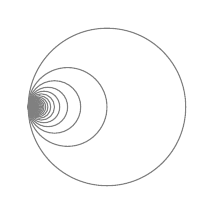
\begin{tikzpicture}
\foreach \n in {1,2,...,100}{
	\draw[gray] ({1/\n},0) circle ({1/\n});
}
\end{tikzpicture}
\end{document}

\end{exampleAndImage}
\begin{example}
The union of all circles with irrational radius passing through the origin and tangent to the vertical axis is even more complicated than the Hawaiian earring.
\end{example}
\begin{lemma}
Any connected finite graph has finitely generated fundamental group.
\end{lemma}
\begin{proof}
Take a connected finite graph \(X\) and a vertex \(x_0 \in X\).
A \emph{tree}\define{tree} is a simply connected graph.
A \emph{maximal subtree}\define{maximal subtree} is a maximal simply connected subgraph; take one, say \(T \subset X\).
Then \(T\) contains all vertices, since otherwise we could add an edge that attaches one more vertex, without creating a loop (any loop would have two edges reaching that vertex).
Each path in \(X\) is determined up to homotopy by listing the edges it passes through.
Each path in \(T\) is uniquely determined, up to homotopy, by its end points, since there is then a unique list of edges giving a path between the end points. 
For each edge \(e_a\) of \(X\) not in \(T\), pick a loop \([x_a]\) in \(X\) starting at \(x_0\), and passing once along \(e_a\).
Every loop \([x]\) in \(X\), starting and ending at \(x_0\), passes finitely many times through each \(e_a\), either in the same direction or the opposite direction to \([x_a]\).
Picture the last edge \(e_a\) which \([x]\) passes along, and picture direction in which it passes.
We can suppose for simplicity that \([x_a]\) traverses \(e_a\) in the opposite direction.
Consider the loop \([y]=[x_a]*[x]\).
It goes through \(e_a\), say through the two vertices \(x_b,x_c\) of \(e_a\), and then passes through \(T\) to \(x_0\), and then back again to \(x_b\) and then \(x_c\).
By uniqueness of paths in \(T\), up to homotopy, with given end points, we can arrange that \([y]\) takes the same route from \(x_c\) to \(x_0\) and then back again.
So \([y]\) is homotopic to cutting that part of \([y]\) out, i.e. up to homotopy \([x_a][x]\) has one fewer pass through \(e_a\) that \([x]\) did.
By induction, we arrange that \([x]\) is a product of these various \([x_a]\).
\end{proof}
\begin{lemma}
Any graph with countably many vertices and edges has countable fundamental group.
\end{lemma}
\begin{proof}
By compactness of \([0,1]\), each loop in the graph can only hit finitely many vertices and so finitely many edges.
Listing the vertices and edges of the loop in order gives the loop up to homotopy.
\end{proof}

\section{More inessential remarks on differential geometry}
A \emph{diffeomorphism}\define{diffeomorphism} is a smooth of manifolds with smooth inverse.
We will not prove:
\begin{theorem}[Sard]
Take a smooth map \(\varphi \colon P \to Q\) of manifolds.
If \(P\) has smaller dimension than \(Q\), then the image of \(\varphi\) is nowhere dense.
If \(P\) and \(Q\) have  equal dimension, there is a dense set of points \(q_0\in Q\) whose preimage \(\varphi^{-1}\set{q_0}\) consists entirely of points \(p_0\in P\) near which \(\varphi\) is a local diffeomorphism.
\end{theorem}
Careful: this point \(q_0\) could have empty preimage, for example if \(\varphi\) maps all of \(P\) to a single point of \(Q\).
\begin{example}
For the spheres \(S^2, S^3, \dots\), any path \(x \colon [0,1] \to S^n\) is smoothly approximated by some smooth path \(y \colon [0,1] \to \R{n+1}\) homotopic to \(x\), which we then divide by \(\norm{y}\) to get a smooth path homotopic to \(x\) lying in \(S^n\).
By Sard's theorem, \(y\) misses some point of the sphere.
Recall that stereographic projection from that point identifies the rest of the sphere with \(\R{n}\), where we can use our previous result to homotope to a constant map: \(\fundamentalGroup{S^n}=\Set{1}\).
Note that this doesn't work for the circle \(S^1\), where the application of Sard's theorem doesn't tell us anything.
\end{example}
A more difficult theorem, which we won't prove, but which may provide some comfort:
\begin{theorem}[Whitney \cite{Hirsch:1994} p. 49 Theorem 2.6]
The smooth maps between any two manifolds are dense in the continuous maps, in the topology of uniform convergence on compact sets, and every continuous map is homotopic to a smooth map.
\end{theorem}

\section{Maps and fundamental groups}
A \emph{diagram}\define{diagram} is a collection of maps between sets, drawn as a graph like:
\[
\begin{tikzcd}[column sep=small, row sep=small]
X \arrow[rr,"f"] \arrow[dr,"g"] & & Z \arrow[dl,"h"] \\
{} & Y & {}
\end{tikzcd}
\]
Start at one of the sets, and follow a path along the maps, in the direction of their arrows: compose those maps.
The diagram \emph{commutes}\define{commutative!diagram}\define{diagram!commutative} if any two paths with the same starting and ending points give the same composition.
In our example, this means that \(g=h \circ f\).

\begin{lemma}
A continuous map \(f \colon X \to Y\) between topological spaces yields a group morphism
\[
f_* \colon \fundamentalGroup{X,x_0} \to \fundamentalGroup{Y,y_0}
\]
where \(y_0=f\of{x_0}\), given by
\[
f_* [x]=[f \circ x]
\]
for any path \(x \colon [0,1] \to X\).
The group morphism doesn't change if \(f\) varies through a homotopy of maps taking \(x_0\) to \(y_0\).
More generally, if we take homotopy \(f_t\) of \(f\) through a family of maps taking, say \(x(t)\) to \(y(t)\), for some paths \(x(t), y(t)=f_t\of{x(t)}\), then there is a commutative diagram between the maps \(f_{0*}\) and \(f_{1*}\):
\[
\begin{tikzcd}
\fundamentalGroup{X,x_0} \arrow{r}{f_0} \arrow{d}{x_*} & \fundamentalGroup{Y,y_0} \arrow{d}{y_*} \\
\fundamentalGroup{X,x_1} \arrow{r}{f_1} & \fundamentalGroup{Y,y_1}
\end{tikzcd}
\]
Under composition of continuous maps
\[
\begin{tikzcd}
X \arrow{r}{f}  & Y \arrow{r}{g} & Z
\end{tikzcd}
\]
the group morphisms 
\[
\begin{tikzcd}
\fundamentalGroup{X,x_0} \arrow{r}{f}  & \fundamentalGroup{Y,y_0} \arrow{r}{g} & \fundamentalGroup{Z,z_0}
\end{tikzcd}
\]
compose: \(\pr{g \circ f}_* = g_* \circ f_*\).
\end{lemma}

A \emph{homotopy equivalence}\define{homotopy!equivalence} is a continuous map \(f \colon X \to Y\) between topological spaces so that there is a continuous map \(g \colon Y \to X\) for which \(f \circ g\) and \(g \circ f\) are both homotopic to identity maps.
A homotopy equivalence identifies fundamental groups.
\begin{example}
The annulus in \(\R{n}\) is homotopy equivalent to the unit sphere, by the map including the sphere into the annulus.
\end{example}
\begin{example}
The sphere in \(\R{n}\) punctured at one point is homotopy equivalent to \(\R{n-1}\) by Ptolemaic projection, and so homotopy equivalent to a point.
\end{example}
\begin{example}
The sphere in \(\R{n}\) punctured at two points is homotopy equivalent to the annulus in \(\R{n-1}\) by Ptolemaic projection, and so to the sphere in \(\R{n-1}\).
\end{example}
\begin{example}
If \(L \subset \R{3}\) is a line, the topological space \(X=\R{3}-L\) is homotopy equivalent to \(S^1\), by projecting to a plane perpendicular to \(L\), punctured where the plane strikes \(L\), and then taking a homotopy to a circle.
\end{example}
\begin{theorem}[Fundamental theorem of algebra]\define{theorem!fundamental, of algebra}\define{algebra!fundamental theorem of}\define{fundamental!theorem of algebra}
Every nonconstant polynomial function of one complex variable has a complex root.
\end{theorem}
\begin{proof}
Take a nonconstant polynomial function 
\[
p(z)=a_0 + a_1 z + \dots + a_n z^n,
\]
with \(a_n \ne 0\).
Clearly \(p(z)\) has a root just where \(p(z)/a_n\) has a root, so we can assume that \(a_n=1\).
Let \(\alpha\) be the maximum of \(|a_0|, |a_1|, \dots, |a_{n-1}|\).
If we pick any \(z\) with \(|z|>(n-1)\alpha\) then clearly the leading term of \(p(z)\) is larger than all other terms added together, so \(p(z) \ne 0\).
Rescale the \(z\) variable if needed to ensure that \((n-1)\alpha<1\).
So if \(|z| \ge 1\) then \(p(z) \ne 0\).
By the same reasoning, none of the functions
\[
p_t(z) = z^n + (1-t)\pr{a_0 + a_1 z + \dots + a_{n-1} z^{n-1}},
\]
vanishes as long as \(|z|\ge 1\), a homotopy betweeen \(p_0(z)=p(z)\) and \(p_1(z)=z^n\).
Let
\[
g_t(e^{i\theta})=\frac{p_t(z)}{p_t(1)},
\]
where \(z=e^{i \theta}\), for \(0 \le t \le 1\).
This map is a homotopy between the loop 
\[
g_0(z) = \frac{p(z)}{p(1)}
\]
with \(z=e^{i\theta}\) and the loop 
\[
g_1(z)=z^n.
\]
Note that \(g_t(1)\) is fixed during the homotopy.

Let
\[
f_t(z)=\frac{p(tz)}{p(t)},
\]
where \(z=e^{i \theta}\) and \(0 \le t \le 1\).
The map \(f\) is a homotopy from the trivial loop at \(t=0\) to a loop at \(t=1\):
\[
f_1(z) =\frac{p(z)}{p(1)} = g_0(z),
\]
for \(z=e^{i\theta}\).
So, inside the plane punctured at the origin, the trivial loop is homotopic to the loop winding \(n\) times and so \(n=0\).
\end{proof}
\begin{problem}{covering.spaces:product.grp}
Prove that the fundamental group of a product is the product of the fundamental groups:
\[
\fundamentalGroup{X \times Y, \pr{x_0,y_0}}
\cong
\fundamentalGroup{X, x_0}
\times
\fundamentalGroup{Y, y_0}.
\]
\end{problem}
\begin{example}
The torus \(T^n=S^1 \times S^1 \times \dots \times S^1\) has fundamental group
\[
\fundamentalGroup{T}=\Z{n}.
\]
\end{example}
\begin{problem}{covering.spaces:horned.sphere}
Give some explanation (not a rigorous proof) why the surface called \emph{Alexander's horned sphere}\define{Alexander's horned!sphere} has uncountable fundamental group, while the open subset of \(\R{3}\) inside (called \emph{Alexander's horned ball}\define{Alexander's horned!ball}) is simply connected.
\begin{center}
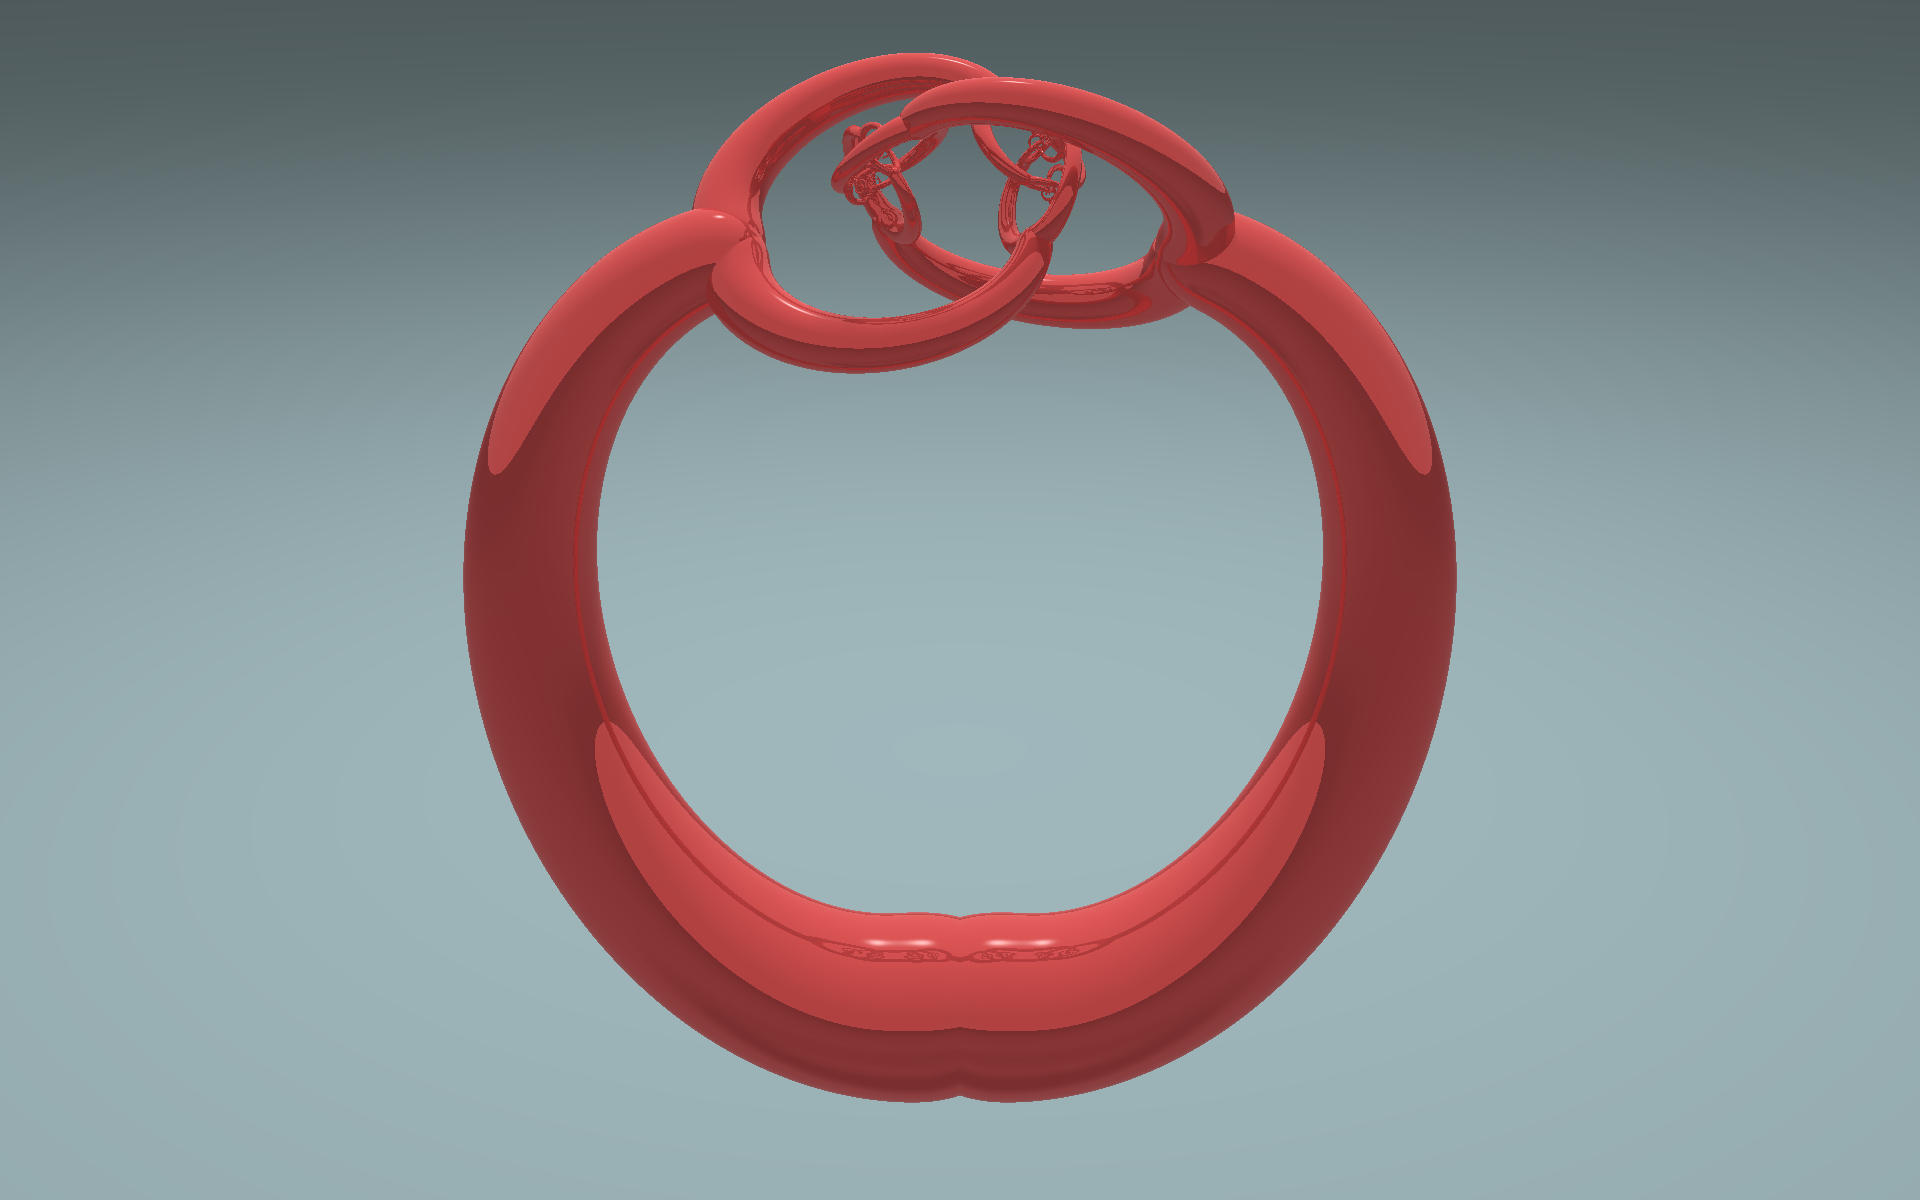
\includegraphics[width=\textwidth]{horned-sphere}
\cprotect\legend{Alexander's horned sphere, Krzysztof Rykaczewski}
\end{center}
\end{problem}
\begin{corollary}\label{corollary:manifolds.countable.pi.1}
If a path connected topological space \(X\) admits a countable basis of simply connected open sets, then its fundamental group is countable.
\end{corollary}
\begin{proof}
The homotopy class of any path is determined by listing off finitely many simply connected open sets that cover it, in the order that it enters them, as in lemma~\vref{lemma:pick.times}.
\end{proof}
\begin{corollary}
Every compact and locally simply connected topological space \(X\) has finitely generated fundamental group.
\end{corollary}
\begin{proof}
By compactness, we can find a finite covering by simply connected open sets \(X_a\) and cover the overlaps \(X_a \cap X_b\) by finitely many path connected open sets \(X'_c\).
The homotopy class of any path is determined by listing off finitely many simply connected open sets that cover it, in the order that it enters them, as in lemma~\vref{lemma:pick.times}.
The homotopy class of any path is determined by listing off finitely many \(X_a\) and \(X'_c\) that cover it, in the order it enters them, as in lemma~\vref{lemma:pick.times}.
\end{proof}
